\subsection{Energy harvesting}\label{sect:background}
\subsubsection{Overview of methods} \label{sect:overview}
This section presents the existing energy harvesting methods. Piezoelectric harvesting and electromagnetic harvesting were found to be most promising and they are studied in greater detail in the following sections.

\begin{description}
  \item[Electromagnetic] methods are based on magnetic induction of electricity \cite{Kubba2014}.
  \item[Electrostatic] harvesting generates power with electrically charged surfaces \cite{Kubba2014}.
  \item[Piezoelectric] materials generate electric power in response to mechanical stress \cite{Kubba2014}.
  \item[Thermal] differences and changes can be converted into electric current \cite{Bowen2014}.
  \item[Triboelectric] materials can generate electricity from friction between tyres \cite{Bowen2014}.
  \item[Radioactive] decay can be used to energise materials for production of power \cite{Lal2004}.
  \item[Photovoltaic] effect can be used to produce electricity from light.
  \item[Radio waves] can be used as a source of energy by utilizing rectenna structures \cite{Patel2014}. 
\end{description}

\textbf{Electromagnetic} power sources are based on Faraday's law of electromagnetic induction. A magnet and a coil are put in motion relative to each other, and the changing magnetic flux through the coils of the generator produces voltage. Current through such device is determined by load resistance. Electromagnetic induction is widely used in power generation, where a primary power source such as wind or flow of water provides rotation for the generator. While conventional designs use rotational movement, linear generator designs exist. Boldea and Nasar \cite{Boldea1999} provide an overview of linear generator and actuator theory. 

\textbf{Electrostatic} devices charge plates of a capacitor and use mechanical vibration to vary the structure of the capacitor. As the capacitance value changes with the structure, energy can be harvested from increased potential energy in capacitor. Drawback of this method is the required control electronics and high polarisation voltages needed for maximal efficiency. There are also electrostatic methods which use \textit{electrets} which hold constant charge and polarisation for years. Electrets can be used in electrostatic harvesters which do not require an external excitation source \cite{Boisseau2012}. However, electret elements and electrostatic generators are not readily available, they have been excluded from this study.

\textbf{Piezoelectric} materials generate charge in response of mechanical stress. This stress can be caused by firmly attaching the piezoelectric element to a surface which deforms (simply supported) or by leaving one end of the element free-hanging while other end is fixed (cantilevered). Dynamics of the generator are very different for the different configurations, Kim et al. \cite{Kim2014a} provides a model for impact-based piezoelectric harvester while Erturk et al. have done in-depth analysis of cantilevered piezoelectric modelling \cite{Erturk2009}. 

\textbf{Thermal} solutions can be further divided into subcategories. A temperature gradient in a semiconductor material causes voltage known as Seebeck-effect in the material. Seebeck-effect is widely used in temperature sensing, but to generate appreciable amounts of power large temperature gradients of over hundred \degree C are required according to study by Amatya et al. \cite{Amatya2010}. Such temperature gradients are not practical inside the tyre. Pyroelectric materials do not require differential of temperature, they generate energy when the temperature of the entire element changes \cite{Zhang2011}. As the temperature inside tyre remains rather constant over long periods of time, these methods are not practical for this application.

\textbf{Triboelectricity} generates power using friction between two materials, a classic example of this is Benjamin Franklin's experiments on charging various rods by rubbing them against different materials. A flexible triboelectric generator has been presented by Fan et al. \cite{Fan2012}. Triboelectric sheets are not readily available and their construction is complex, so triboelectric generation is excluded from this work. 

\textbf{Magnetostrictive} materials change their magnetic field in response to external mechanical stress. This change can be utilised to create a magnetic flux through coils as in electromagnetic generators. A magnetostrictive generator was built by Wang et al. \cite{Wang2006}. 

Solar energy can be harvested by using sun as a energy source for a thermal energy harvesting or by utilising the \textbf{photovoltaic} (PV) effect to generate electricity from photons hitting PV material. PV technology is mature and widely used, and PV cells attached to the rim of a tyre could produce ample power during summertime. PV cells would however incur extra maintenance as the rims would have to be cleaned whenever power output falls. 

\textbf{Radio wave} harvesting uses antennas to collect energy from ambient radio transmissions, such as WiFi- and cellular signals. Patel et al \cite{Patel2014} have built a demonstration device which uses TV broadcasts as an energy source. The tyre material dampens any Radio frequency (RF) broadcasts, which makes RF energy harvesting poorly suited for this application.

\textbf{Radioactive} energy harvesting resembles battery or fuel cell. A radioactive material is deposited in generator near piezoelectric cantilever. Radioactive decay charges proof mass of piezoelectric cantilever until the proof mass contacts the radioactive material by electrostatic attraction, at which point the electrical charge is balanced and piezoelectric beam begins resonant vibration as in normal piezoelectric harvesting. Such a battery has lifetime limited only by half-life of the used material. Lal and Blanchard \cite{Lal2004} present such a battery. This kind of battery would be redundant for this application, as there already exists energy in rotation of tyre which can be used to energise the cantilever. 

In conclusion, this section has presented wide range of energy harvesting technologies. As their primary properties are known, most promising technologies for car tyre energy harvesting can be narrowed to \textbf{electromagnetic} and \textbf{piezoelectric}. These technologies are studied further in the following sections to identify optimal choice for the application.

\subsubsection{Resonance-based piezoelectric harvesting}
Resonant piezoelectric harvesters are presented in deeper detail in this section. The 

Piezoelectric materials produce voltage in response to mechanical stress. The effect is bidirectional, piezoelectric element can also produce mechanical strain in response to applied voltage. The material has crystalline structure with electrical dipoles in balanced state when no stress is applied. Mechanical stress unbalances these dipoles, creating element which electronically resembles a charged capacitor. 

A common approach to piezoelectric harvesting is to configure the element as a cantilever and tune the resonant frequency of the system to dominant frequency of the surrounding environment. This kind of system is shown in Figure \ref{fiq:resonant_piezo}. In some applications, such as in machines running at the frequency of power grid (50 Hz or 60 Hz) this kind of frequency-tuning is relatively straightforward.

\begin{figure}[htb]
  \begin{center}
  \includegraphics[height=6cm]{images/cited/arroyo2012}
  \end{center}
  \caption{Piezoelectric generator configured as cantilever by Arroyo et al. \cite{Arroyo2012}.}
  \label{fiq:resonant_piezo}
\end{figure}

This kind of resonant harvesting is challenging in a tyre. The energy harvester has a very sharp peak efficiency frequencies, and dominant frequency of tyre varies with the speed of the car. On the other hand, there is almost guaranteed broadband energy available from moments where the tyre contacts road. There is also some research on tuning the resonant frequency of cantilevered piezoelectric harvester by Singh et al \cite{Singh2012}. They used intelligently driven Switch-Mode Power Supply (SMPS) to impedance-match the load to a piezoelectric element. As the electro-mechanical nature of piezoelement means changing load changes the mechanical properties of the piezoelement, resonance frequency can track the dominant frequency of system within some limits. Figure \ref{fiq:tracking_piezo} shows the tracking behaviour Singh et al. achieved, resonance can be adjusted in range of 65 - 70 Hz.

\begin{figure}[htb]
  \begin{center}
  \includegraphics[height=8cm]{images/cited/singh2012}
  \end{center}
  \caption{Frequency tuning results by Singh et al \cite{Singh2012}.}
  \label{fiq:tracking_piezo}
\end{figure}

The results of Singh et al. can be considered as the state of art for resonance-based piezoelectric harvesting in tyre, and their power output was around 40 $\mu W$ at peak efficiency. An estimate of energy needs of tyre sensor is given in Section \ref{sect:power_requirement}, 40 $\mu W$ exceeds energy required by the sleep mode of proposed sensor.

In conclusion, resonant piezoelectric harvesting is not optimal for car tyre application, as the resonant frequency is fixed and any dynamic tracking capacity is limited. Therefore, impact-based piezoelectric harvesting is studied in next section.

\subsubsection{Impact-based piezoelectric harvesting}
Previous section concluded resonant harvesting is not optimal method for the environment of this application. Another method would be to use an impactor to hit a piezoelectric plate on the tyre. These impacts would provide energy once per rotation. This method has been experimented with before by Manla et al \cite{Manla2009}. Their generator produced 4 $mW$ electrical power.

Piezoelectric elements are often electrically modelled as current source with parallel capacitor or a voltage source with series capacitor, as shown in figure \ref{fig:piezo_equivalents} by Kanda et al \cite{Kanda2012}. There are also a lot more complex models which account for mechanical phenomena in piezoelement, as well as loading effects coupling on mechanical model. For the purposes of model identification for the piezo only simplest voltage source (a) and current source (b) models are explored.

\begin{figure}[htb]
  \begin{center}
  \includegraphics[height=6cm]{images/cited/kanda2012}
  \end{center}
  \caption{Electrical equivalent models for piezoelectric element \cite{Kanda2012}.}
  \label{fig:piezo_equivalents}
\end{figure}

The model (b) in Figure \ref{fig:piezo_equivalents} shows clearly that no DC current can flow in or out of piezo element. Maximum current in any cycle of a piezoelement is limited by the open loop voltage which is seen on the terminals of the piezoelement and piezo capacitance in series with circuit. 

The implication for impact-based harvesting is somewhat discouraging: total amount of power obtainable is limited by the frequency of impacts. However, if there is any natural resonance frequency for the piezo generator, some of the energy in the impact should be in appropriate spectrum for the generator and the generator could produce decaying amount of power in-between of the impacts.

\subsubsection{Electromagnetic harvesting} \label{sect:em_harvest}
Electromagnetic harvesting is based on Faraday's law of induction: A loop of wire acquires electromotive force (EMF) in response to a changing magnetic field. More formally:

\begin{equation}
  \varepsilon = - \frac{d \Phi_ {B}}{d t} , 
\end{equation}
where $\varepsilon$ is the EMF, $\Phi_{B}$ is magnetic flux through loop area, and $t$ is time. Negative sign signifies that the EMF opposes the change of magnetic flux. For a tightly wound coil of wire, the equation can be stated as: 

\begin{equation} \label{eq:emf}
  \varepsilon = -N_{turns} \frac{d \Phi_{B}}{d t} , 
\end{equation}
where $N_{turns}$ is the number of turns in a coil \cite[p.998]{universityphysics}.

It's important to notice that magnetic flux through wire $ \Phi_{B} $ can change for a variety of reasons: the source of field can be in motion, strength of the field can vary, the coil can be in motion, and the shape of coil can vary. In an energy harvesting application in an environment with vibrations motional energy is readily available, so we focus on energy harvesting methods which either move the source of magnetic field or the coil itself.

It can be determined from the Equation \eqref{eq:emf} that the energy available increases with the strength of magnetic source, number of turns in a coil and rate of change in the magnetic field. 

The magnetic source can be either a permanent magnet or an electrically induced source as in induction motors. Induction-based generators require reactive power to start up, which means that any harvester design incorporating an induction generator would need a secondary power source to start the inductive generator. Secondary power source would have to be a battery, which would defeat the purpose of avoiding batteries on the design. Hence the focus of this thesis will be in the permanent magnet designs.

In addition to the voltage available from the generator, it's important to consider the source impedance. A very simple electrical equivalent model of the generator is presented in Figure \ref{gen_simple}, where generator is presented as a voltage source in series with lumped inductor and resistor \cite{Jirutitijaroen2012}. 

\begin{figure}[htb]
\begin{center}
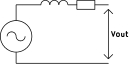
\includegraphics[height=2cm]{images/own_dwg/gen_simple}
\end{center}
\caption{A simple electromechanical generator equivalent circuit. Coil inductance and resistance are modeled as lumped components in series with EMF modeled as voltage source.}
\label{gen_simple}
\end{figure}

This model is greatly simplified and it does not account for factors such as the effect of electromagnetic force on mechanical structure of the generator. Even with these limitations, the model is still useful as it can be used to determine the optimal load for the generator. 

The power output can be written formally as:

\begin{equation} \label{eq:gen_simple_power}
  P_{generated}(s) = \varepsilon(s) \cdot I_{generated}(s),
\end{equation}
where $P_{generated}(s), \varepsilon(s), I_{generated}(s)$ are complex frequency-domain power, voltage and current. Voltage is determined by EMF as described above. Current can be written as: 

\begin{equation} \label{eq:gen_simple_current}
  I_{generated}(s) = \frac{\varepsilon(s)}{Z_{generator}(s)+Z_{load}(s)},
\end{equation}
where $Z_{generator}(s) $ and $ Z_{load}(s)$ are complex impedances of load and generator. This equation is valid only for linear systems, so for example rectifying and converting power with a SMPS reduces accuracy of the equation. Substituting Equation \eqref{eq:gen_simple_current} into Equation \eqref{eq:gen_simple_power} we obtain:

\begin{equation}
  P_{generated}(s) = \varepsilon(s) \cdot \frac{\varepsilon(s)}{Z_{generator}(s)+Z_{load}(s)}.
\end{equation}
Total power into load can be written as:

\begin{equation} \label{eq:generator_load_power}
  P_{load}(s) = \varepsilon(s)  \cdot  \frac{Z_{load}(s)}{Z_{generator}(s)+Z_{load}(s)}  \cdot  \frac{\varepsilon(s)}{Z_{generator}(s)+Z_{load}(s)}.
\end{equation}
It's easy to see from the Equation \eqref{eq:generator_load_power} that if the load impedance is infinite or zero, there is no power generated. It can be shown that maximum power is generated when load impedance is complex a conjugate of generator impedance, $Z_{generator}(s) = {Z_{load}(s)}^*$. Another issue to consider is the efficiency of the generator: the electrical efficiency is defined as a ratio of the power flowing into the load and the total power generated. The equation \eqref{eq:generator_load_power} can be used to show that when the load impedance is equal to the generator impedance, efficiency is $ 50 \%$. The efficiency rises with the load impedance, which is why generators are rarely run at their maximum power. In our application the harvested power is minuscule compared to power available in the tyre, so it is reasonable to try to match the load impedance for maximum power.

In an energy harvesting application, it is important to consider the validity of the established theory when a generator is scaled to centimetres or even smaller dimensions. Many assumptions, such as a coil being tightly wound and made of thin wire might become invalid at microscale. O'Donnel et al. \cite{ODonnell2007} have done a study on the effects of scaling dimensions downwards down to millimetre range, and they concluded that power available from the generator is proportional to the fourth power of generator dimension for cubical generators. Another of their primary findings was that a microfabricated generator becomes more effective than a traditional wire-wound generator when design is scaled below $2 mm$ length or in $8 mm^3$ volume. It can be concluded that in this application it is reasonable to use a wire-wound generator over a microfabricated one, as the generator dimensions can be an order of magnitude larger than this crossover point. 


\subsection{Structure of a tyre}

Tyres are composed of several layers with different functions. Figure \ref{fig:tyre_structure_diagram} by Gent et al. \cite{Gent2005} shows the layered structure. From outer tread to inner lining, the layers are: 

\begin{description}
  \item[Tread] is the outer profile of tyre which provides traction for driving, braking and cornering. Pattern and materials on
tread is a compromise between wear resistance, traction, handling and rolling
resistance.
  \item[Belts] are inner structural supports that provide mechanical strength, impact resistance and keep tyre from expanding
under centrifugal forces.
  \item[Body ply] is a sheet which provides strength to contain the air pressure.
  \item[Innerliner] is a compound specifically designed to improve air retention in tyre.
\end{description}
In addition there are layers designed to improve tyre reliability, such as the belt
wedge which reduces shear between belts. 


\begin{figure}[h]
\begin{center}
\includegraphics[height=8cm]{images/cited/gent2005}
\end{center}
\caption{Structure of a tyre \cite{Gent2005}.}
\label{fig:tyre_structure_diagram}
\end{figure}


In endurance testing of tyres, a car is driven at a test track until
a desired number of course driving kilometres have been reached. In outdoor testing
each company has their own proprietary test protocol. Indoor testing has standards
which mandate pressure, ambient temperature and speed as well as time driven.
According to Gent et al. \cite{Gent2005} this standard indoor testing takes 34 hours of driving at 120
km / h.

In addition to endurance testing, there is high-speed testing where tyre speed is
gradually accelerated in steps of 10 km / h at regular intervals until the target speed is
reached. Energy harvester should survive these tests to be considered a viable design for road conditions.


\subsection{Environment inside tyre} \label{sect:tyre_environment}
The energy harvester will be placed inside a tyre. Therefore knowledge of the environment inside the tyre is required for intelligent design of a harvester. This section presents the acceleration and mechanical characteristics inside tyre. 

The tyre will experience acceleration in all three axes\cite{Niskanen2014}. Tangential and centripetal accelerations are dominant, they can reach amplitudes up to 150 g in test fixture. In addition a study done by Löhndorf et al. \cite{Lohndorf2007} shows shock survival of up to 4 000 - 5 000 g is required for reliability. 

Temperature inside the tyre will reach an equilibrium in ambient + 5 ... 10 \degree C, so operation temperature should be in range of -40 to + 75 \degree C to have some safety margin on top of usual ambient conditions. 

Previous work by Niskanen et al. \cite{Niskanen2014} was used as a basis for analysis of characteristics of acceleration inside the tyre. Raw data from their study was used to determine minimum and maximum values of acceleration as well as frequency components of acceleration inside tyre. Data was gathered at 20 km/h, 60 km/h and 80 km/h speeds. Figure \ref{80_TD} shows time domain amplitude of the acceleration along 3 axes as shown in Figure \ref{tyre_axes}.

\begin{figure}[htb]
\begin{center}
\includegraphics[height=4cm]{images/cited/matilainen2012}
\end{center}
\caption{Axes in measurement defined by Matilainen et al. \cite{Matilainen2012}}
\label{tyre_axes}
\end{figure}

Frequency domain representations were calculated in Matlab. There are two main contributors to base frequencies: first is the rotational frequency of tyre itself and second is the impact when the tyre deforms as it contacts the drum.. There is clearly visible series of frequency components spaced at the rotational frequency of tyre as well as shock harmonics at upper frequencies. Figure \ref{80_FFT_zoom} shows the total frequency spectrum and the dominant frequency components.

\begin{figure}[htb]
\begin{center}
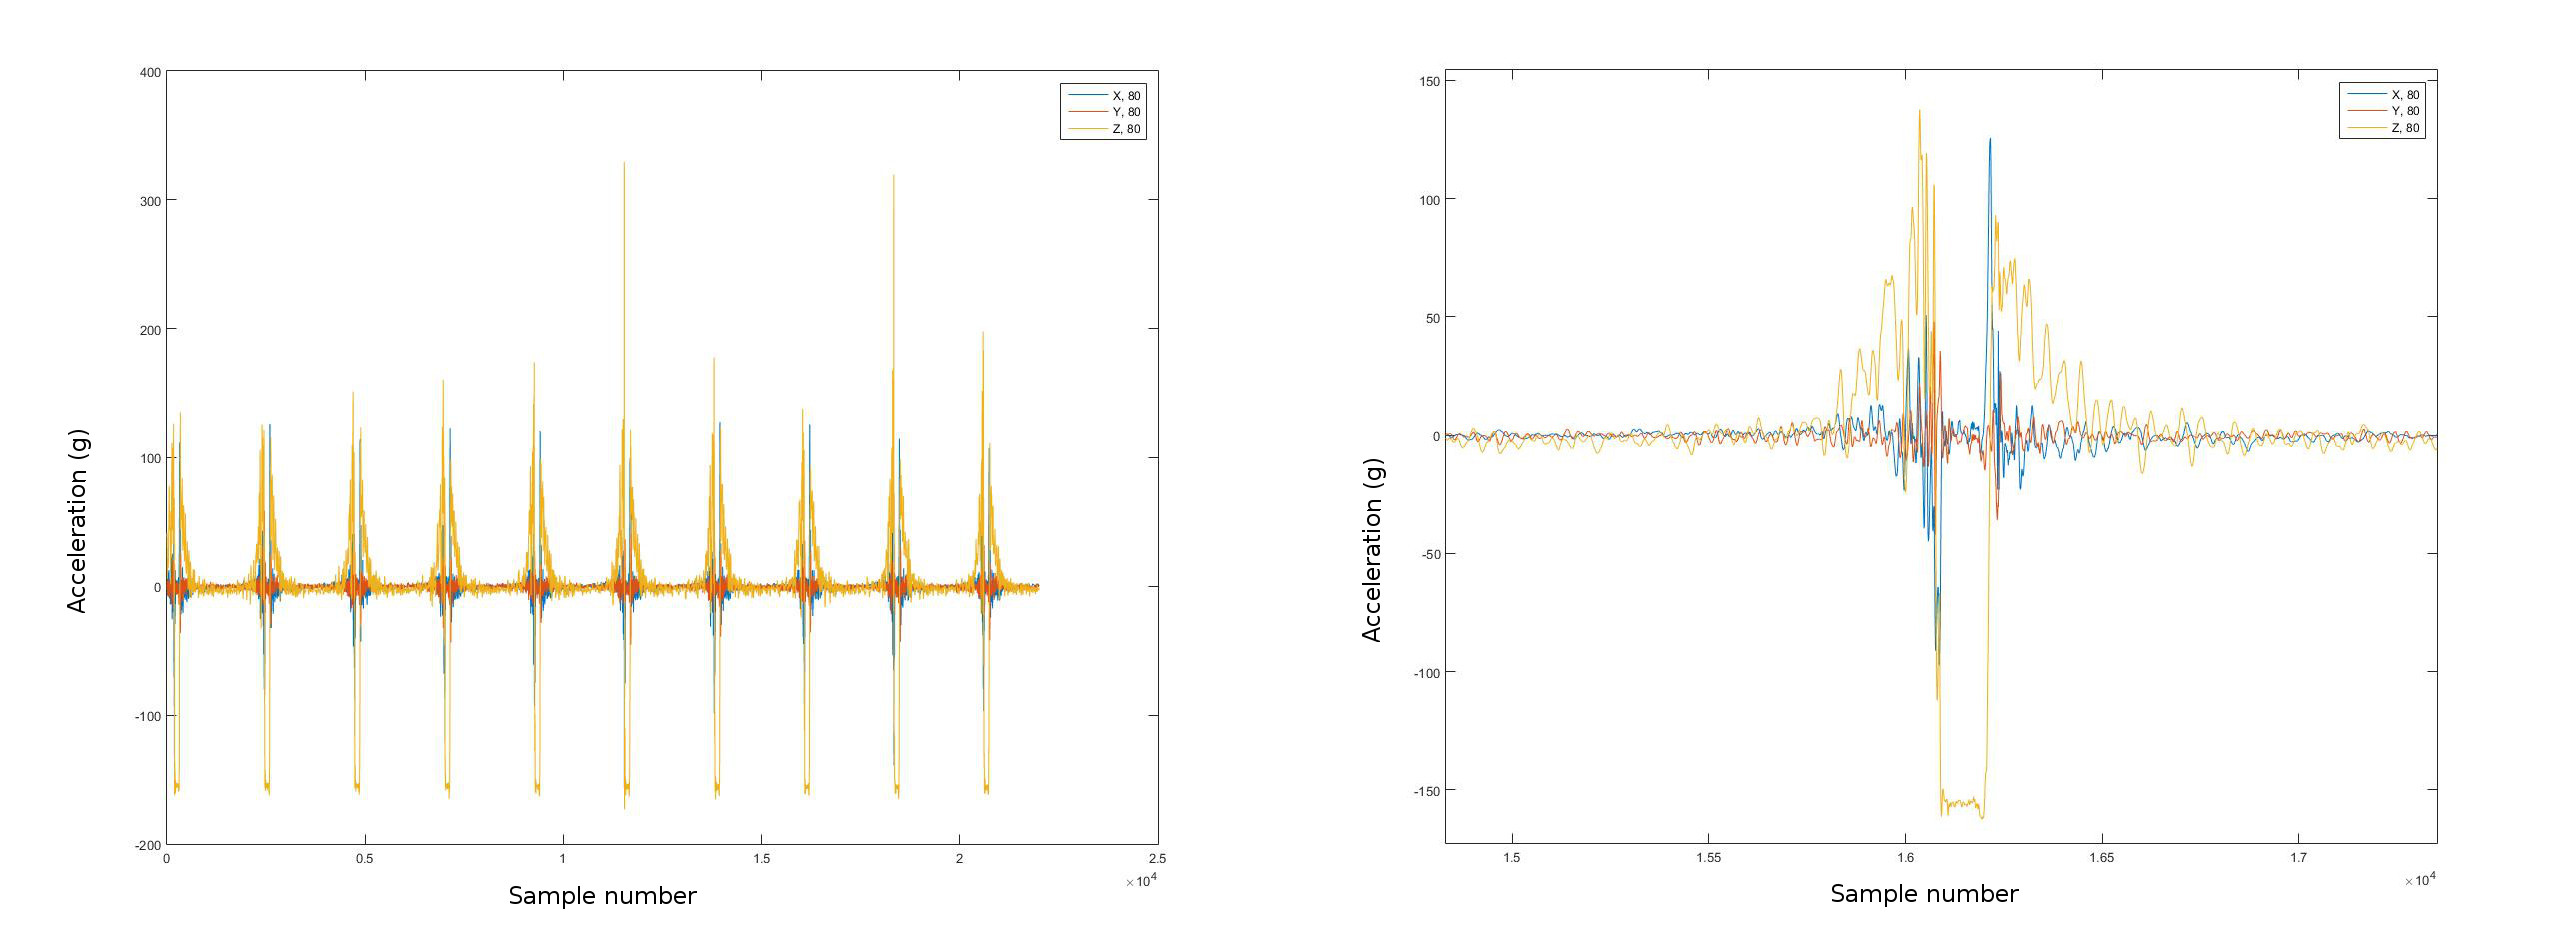
\includegraphics[width=\columnwidth]{images/matlab_figures/80kmh_timedomain_combined}
\end{center}
\caption{Acceleration of inner lining of tyre at 80 km/h in time domain.}
\label{80_TD}
\end{figure}

\begin{figure}[htb]
\begin{center}
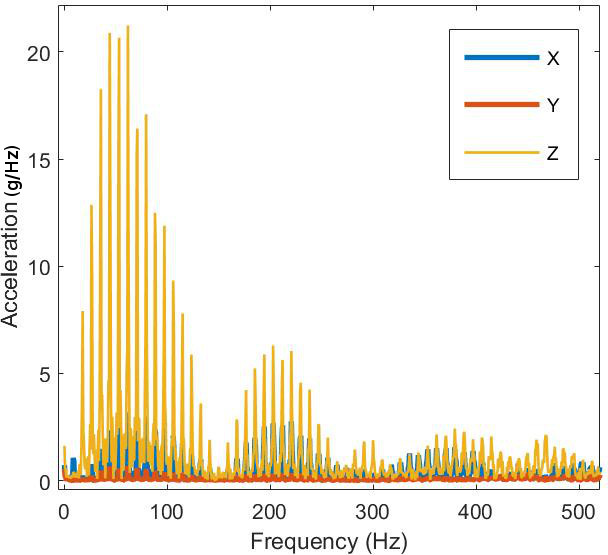
\includegraphics[height=6cm]{images/matlab_figures/fft.jpg}
\end{center}
\caption{Most of the energy is found in 10-100 Hz range.}
\label{80_FFT_zoom}
\end{figure}

It's important to notice that the sensor used was piezoelectric, which forms a highpass filter as the operation of sensor is based on charge between layers. This charge dissipates over time, so the steady-state centripetal acceleration reads as zero. Any device on the rotating tyre will experience centripetal acceleration (acceleration toward centre of rotation) at the amplitude of: 

\begin{equation}
  a_{centripetal} = \omega^2 r,
\end{equation}
where $\omega$ is the rotation speed of tyre and $r$ is the radius of rotation.

The tyre structure deforms during the contact with the road. A study by Xiong et al. \cite{Xiong2014} shows the tyre can compress over 2 cm during contact to road in normal driving conditions as shown in Figure \ref{fig:deformation}. The compression can be even greater if the tyre has low internal pressure. 

\begin{figure}[htb]
    \begin{center}
    \includegraphics[width=\columnwidth]{images/cited/xiong2014.jpg}
    \end{center}
    \caption{\label{fig:deformation} The tyre radius change in one full rotation measured by the optical tyre sensor. \cite{Xiong2014}}
\end{figure}

The tyre deformation causes two distinct challenges for mechanical design of harvester: first, the deformation limits maximum height of harvester to avoid mechanical contact between rim and the harvester top. Second challenge is in the mounting, as harvester the base must survive deformation. In conclusion, tyre operational environment causes significant challenges for long term reliability of any device mounted inside the surface of tyre. 
